\section{Geom\-PQP  Class Reference}
\label{classGeomPQP}\index{GeomPQP@{Geom\-PQP}}
Parent class PQP-based list of Triangle models. 


{\tt \#include $<$geom\-PQP.h$>$}

Inheritance diagram for Geom\-PQP::\begin{figure}[H]
\begin{center}
\leavevmode
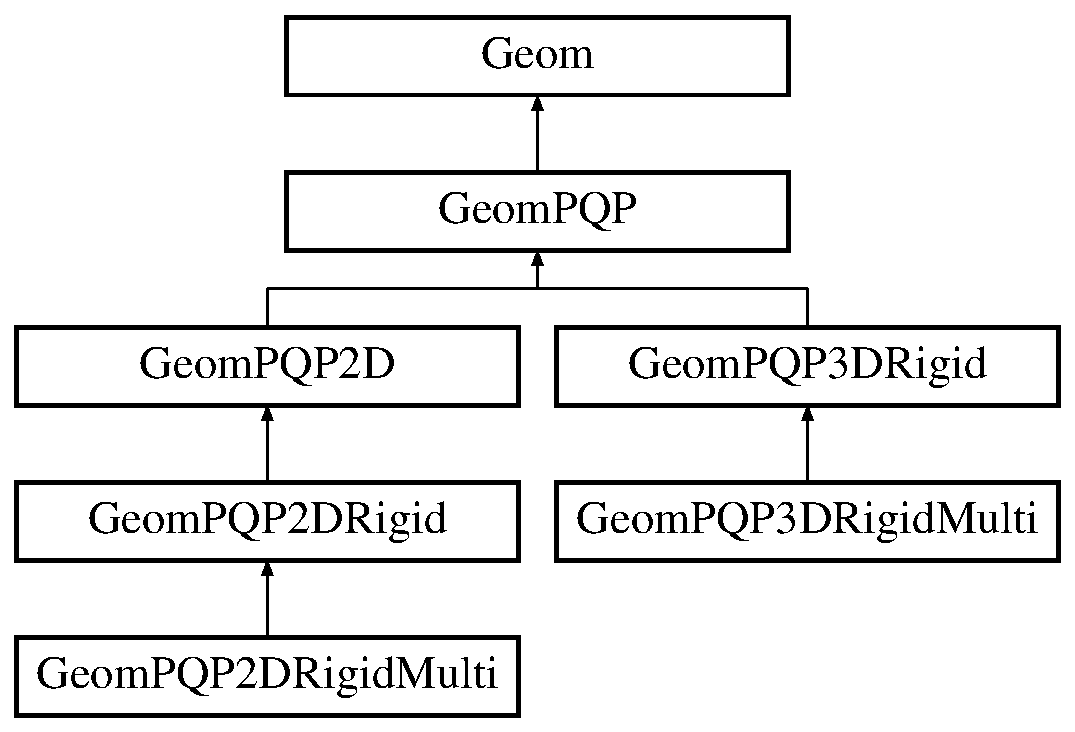
\includegraphics[height=5cm]{classGeomPQP}
\end{center}
\end{figure}
\subsection*{Public Methods}
\begin{CompactItemize}
\item 
{\bf Geom\-PQP} (string path)
\item 
virtual {\bf $\sim$Geom\-PQP} ()
\item 
virtual void {\bf Load\-Environment} (string path)
\item 
virtual void {\bf Load\-Robot} (string path)
\item 
virtual bool {\bf Collision\-Free} (const {\bf MSLVector} \&q)
\begin{CompactList}\small\item\em Return true if the robot(s) and obstacles are not in collision.\item\end{CompactList}\item 
virtual double {\bf Distance\-Comp} (const {\bf MSLVector} \&q)
\begin{CompactList}\small\item\em Compute the distance of the closest point on the robot to the obstacle region.\item\end{CompactList}\end{CompactItemize}
\subsection*{Public Attributes}
\begin{CompactItemize}
\item 
list$<$ {\bf MSLTriangle} $>$ {\bf Obst}
\item 
list$<$ {\bf MSLTriangle} $>$ {\bf Robot}
\item 
PQP\_\-Model {\bf Ro}
\item 
PQP\_\-Model {\bf Ob}
\end{CompactItemize}
\subsection*{Protected Attributes}
\begin{CompactItemize}
\item 
PQP\_\-REAL {\bf RR} [3][3]
\item 
PQP\_\-REAL {\bf RO} [3][3]
\item 
PQP\_\-REAL {\bf TR} [3]
\item 
PQP\_\-REAL {\bf TO} [3]
\end{CompactItemize}


\subsection{Detailed Description}
Parent class PQP-based list of Triangle models.



\subsection{Constructor \& Destructor Documentation}
\index{GeomPQP@{Geom\-PQP}!GeomPQP@{GeomPQP}}
\index{GeomPQP@{GeomPQP}!GeomPQP@{Geom\-PQP}}
\subsubsection{\setlength{\rightskip}{0pt plus 5cm}Geom\-PQP::Geom\-PQP (string {\em path})}\label{classGeomPQP_a0}


\index{GeomPQP@{Geom\-PQP}!~GeomPQP@{$\sim$GeomPQP}}
\index{~GeomPQP@{$\sim$GeomPQP}!GeomPQP@{Geom\-PQP}}
\subsubsection{\setlength{\rightskip}{0pt plus 5cm}virtual Geom\-PQP::$\sim$Geom\-PQP ()\hspace{0.3cm}{\tt  [inline, virtual]}}\label{classGeomPQP_a1}




\subsection{Member Function Documentation}
\index{GeomPQP@{Geom\-PQP}!CollisionFree@{CollisionFree}}
\index{CollisionFree@{CollisionFree}!GeomPQP@{Geom\-PQP}}
\subsubsection{\setlength{\rightskip}{0pt plus 5cm}virtual bool Geom\-PQP::Collision\-Free (const {\bf MSLVector} \& {\em q})\hspace{0.3cm}{\tt  [inline, virtual]}}\label{classGeomPQP_a4}


Return true if the robot(s) and obstacles are not in collision.



Implements {\bf Geom} {\rm (p.\,\pageref{classGeom_a2})}.

Reimplemented in {\bf Geom\-PQP2DRigid} {\rm (p.\,\pageref{classGeomPQP2DRigid_a2})}.\index{GeomPQP@{Geom\-PQP}!DistanceComp@{DistanceComp}}
\index{DistanceComp@{DistanceComp}!GeomPQP@{Geom\-PQP}}
\subsubsection{\setlength{\rightskip}{0pt plus 5cm}virtual double Geom\-PQP::Distance\-Comp (const {\bf MSLVector} \& {\em q})\hspace{0.3cm}{\tt  [inline, virtual]}}\label{classGeomPQP_a5}


Compute the distance of the closest point on the robot to the obstacle region.



Implements {\bf Geom} {\rm (p.\,\pageref{classGeom_a3})}.

Reimplemented in {\bf Geom\-PQP2DRigid} {\rm (p.\,\pageref{classGeomPQP2DRigid_a3})}.\index{GeomPQP@{Geom\-PQP}!LoadEnvironment@{LoadEnvironment}}
\index{LoadEnvironment@{LoadEnvironment}!GeomPQP@{Geom\-PQP}}
\subsubsection{\setlength{\rightskip}{0pt plus 5cm}void Geom\-PQP::Load\-Environment (string {\em path})\hspace{0.3cm}{\tt  [virtual]}}\label{classGeomPQP_a2}




Reimplemented in {\bf Geom\-PQP2D} {\rm (p.\,\pageref{classGeomPQP2D_a2})}.\index{GeomPQP@{Geom\-PQP}!LoadRobot@{LoadRobot}}
\index{LoadRobot@{LoadRobot}!GeomPQP@{Geom\-PQP}}
\subsubsection{\setlength{\rightskip}{0pt plus 5cm}void Geom\-PQP::Load\-Robot (string {\em path})\hspace{0.3cm}{\tt  [virtual]}}\label{classGeomPQP_a3}




Reimplemented in {\bf Geom\-PQP2D} {\rm (p.\,\pageref{classGeomPQP2D_a3})}.

\subsection{Member Data Documentation}
\index{GeomPQP@{Geom\-PQP}!Ob@{Ob}}
\index{Ob@{Ob}!GeomPQP@{Geom\-PQP}}
\subsubsection{\setlength{\rightskip}{0pt plus 5cm}PQP\_\-Model Geom\-PQP::Ob}\label{classGeomPQP_m3}


\index{GeomPQP@{Geom\-PQP}!Obst@{Obst}}
\index{Obst@{Obst}!GeomPQP@{Geom\-PQP}}
\subsubsection{\setlength{\rightskip}{0pt plus 5cm}list$<${\bf MSLTriangle}$>$ Geom\-PQP::Obst}\label{classGeomPQP_m0}


\index{GeomPQP@{Geom\-PQP}!Ro@{Ro}}
\index{Ro@{Ro}!GeomPQP@{Geom\-PQP}}
\subsubsection{\setlength{\rightskip}{0pt plus 5cm}PQP\_\-Model Geom\-PQP::Ro}\label{classGeomPQP_m2}


\index{GeomPQP@{Geom\-PQP}!RO@{RO}}
\index{RO@{RO}!GeomPQP@{Geom\-PQP}}
\subsubsection{\setlength{\rightskip}{0pt plus 5cm}PQP\_\-REAL Geom\-PQP::RO[3][3]\hspace{0.3cm}{\tt  [protected]}}\label{classGeomPQP_n1}


\index{GeomPQP@{Geom\-PQP}!Robot@{Robot}}
\index{Robot@{Robot}!GeomPQP@{Geom\-PQP}}
\subsubsection{\setlength{\rightskip}{0pt plus 5cm}list$<${\bf MSLTriangle}$>$ Geom\-PQP::Robot}\label{classGeomPQP_m1}


\index{GeomPQP@{Geom\-PQP}!RR@{RR}}
\index{RR@{RR}!GeomPQP@{Geom\-PQP}}
\subsubsection{\setlength{\rightskip}{0pt plus 5cm}PQP\_\-REAL Geom\-PQP::RR[3][3]\hspace{0.3cm}{\tt  [protected]}}\label{classGeomPQP_n0}


\index{GeomPQP@{Geom\-PQP}!TO@{TO}}
\index{TO@{TO}!GeomPQP@{Geom\-PQP}}
\subsubsection{\setlength{\rightskip}{0pt plus 5cm}PQP\_\-REAL Geom\-PQP::TO[3]\hspace{0.3cm}{\tt  [protected]}}\label{classGeomPQP_n3}


\index{GeomPQP@{Geom\-PQP}!TR@{TR}}
\index{TR@{TR}!GeomPQP@{Geom\-PQP}}
\subsubsection{\setlength{\rightskip}{0pt plus 5cm}PQP\_\-REAL Geom\-PQP::TR[3]\hspace{0.3cm}{\tt  [protected]}}\label{classGeomPQP_n2}




The documentation for this class was generated from the following files:\begin{CompactItemize}
\item 
{\bf geom\-PQP.h}\item 
{\bf geom\-PQP.C}\end{CompactItemize}
